\documentclass[9pt]{beamer}
\usepackage[english]{babel}
\usetheme{default}
\usepackage{datetime}
\usepackage{adjustbox}
\usepackage{amsmath}
\usepackage{mathtools}
\usepackage{listings}
\usepackage{hyperref}
\usepackage{amsmath}
\usepackage{amssymb}
\usepackage{multicol}
\usepackage{multirow}
\usepackage{setspace}
\usepackage{algorithmic, algorithm}
\newcommand\tab[1][5mm]{\hspace*{#1}}

\newdate{date}{24}{01}{2024}

\title{\Large Verification of Binarized Neural Networks using alpha-beta-CROWN and Marabou}

\author{Rafael-Valentin Ban, Cosmin-\c Stefan Negureanu, Mihai-Iosif F\^{a}r\c tal\u a, Cristina-Larisa Petcu, M\u ad\u alina-Maria Radu}

\institute{West University of Timi\c soara\\Faculty of Mathematics and Informatics

Master Study Program: Software Engineering

\bigskip

Coordinator: Conf. Dr. M\u ad\u alina Era\c scu}

\date{\small{\displaydate{date}}
	
\bigskip

\begin{center}

\includegraphics[height=1.0cm]{FMI-03.png}
\end{center}
}

\AtBeginSubsection[]
{
  \begin{frame}[t]<beamer>{Overview}
    \tableofcontents[currentsection,currentsubsection]
  \end{frame}
}

\begin{document}
\begin{frame}[t]
  \titlepage
\end{frame}
\begin{frame}[t]{Overview}
  \tableofcontents
\end{frame}

\section{Introduction}
\begin{frame}[plain,c]{Introduction}
\setstretch{3} 
\begin{itemize}
    \item Motivation
    \begin{itemize}
        \item Improving verification rates of benchmark
    \end{itemize}
    \item Problem specification
    \begin{itemize}
        \item Self-driving
        \item Neural networks tool verifiers versus real life testing
    \end{itemize}
\end{itemize}
\end{frame}
\section{Dataset description}
\begin{frame}[plain,c]{Dataset description}
\begin{figure}[h]
\centering
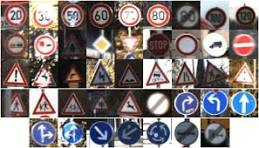
\includegraphics[scale=0.8]{figure2.jpg}
\caption{Some images used in the German Traffic Signs Recognition Benchmark}
\end{figure}
\end{frame}
\begin{frame}[plain,c]{Dataset description}
\begin{figure}[h]
\centering
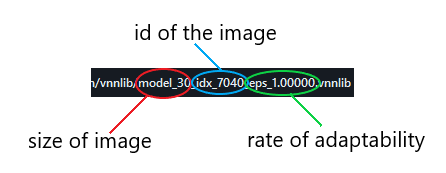
\includegraphics[scale=0.8]{figure3.png}
\caption{Properties file used for verification}
\end{figure}
\end{frame}

\section{Tools}
\begin{frame}[plain,c]{Tools}
\setstretch{3} 
\begin{itemize}
    \item alpha-beta-CROWN
    \begin{figure}[h]
    \centering
    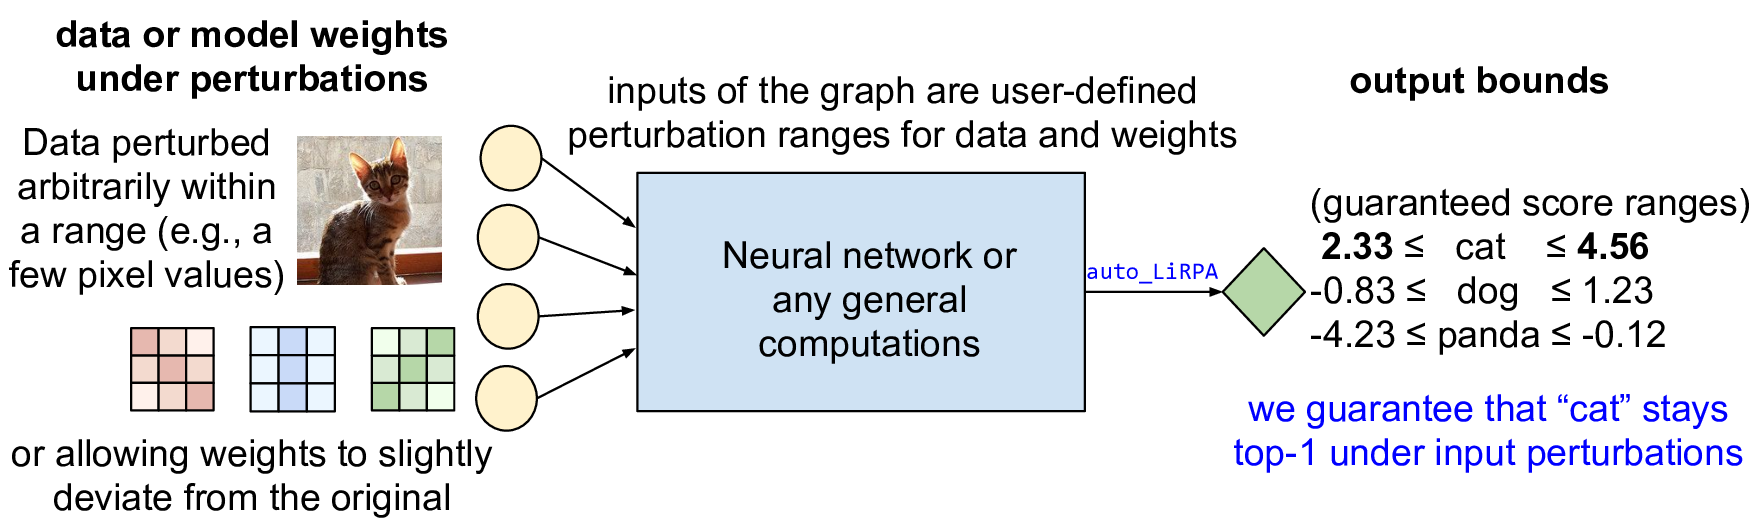
\includegraphics[scale=0.17]{figure4.png}
    \caption{Rough explanation of efficient linear bound propagation}
    \end{figure}
\end{itemize}
\end{frame}
\begin{frame}[plain,c]{Tools}
\setstretch{3} 
\begin{itemize}
    \item Marabou
\end{itemize}
\end{frame}

\section{Experimental Results}
\begin{frame}[plain,c]{Experimental Results}
\begin{center}
\begin{tabular}{ c c c c c c}
 \hline
 \textbf{\#} & \textbf{Tool} & \textbf{Verified} & \textbf{Falsified} & \textbf{Penalty}\\
 \hline
 1 & alpha-beta-CROWN & 0 & 39 & 3\\
 \hline
 2 & Marabou & - & - & -\\
 \hline
 3 & Nnenum & 0 & 0 & 46\\
 \hline
\end{tabular}
\end{center}
\end{frame}

\section{Conclusion}
\begin{frame}[plain,c]{Conclusion}
\setstretch{3} 
\begin{itemize}
    \item Posibility of verification improvement exists.
    \item Image verification is hard!
\end{itemize}
\end{frame}

\section{Demo}
\begin{frame}[plain,c]{Demo}
\setstretch{3} 
\begin{itemize}
    \item alpha-beta-CROWN\\
    \url{https://www.youtube.com/watch?v=cXHRKEpAh78}
    \item Marabou \& Nnenum\\
    \url{https://www.youtube.com/watch?v=YZIZdvPJcC8}
\end{itemize}
\end{frame}
\end{document} 